\section{Durchführung}
\label{sec:Durchführung}

Der Versuch wird nach \autoref{fig:aufbauSch} aufgebaut. Um die Frank-Hertz Kurven aufzuzeichnen wird ein XY-Schreiber verwendet. Die Temperaturregelung erfolgt über ein separates Heizgerät.

\begin{figure}[H]
    \centering
    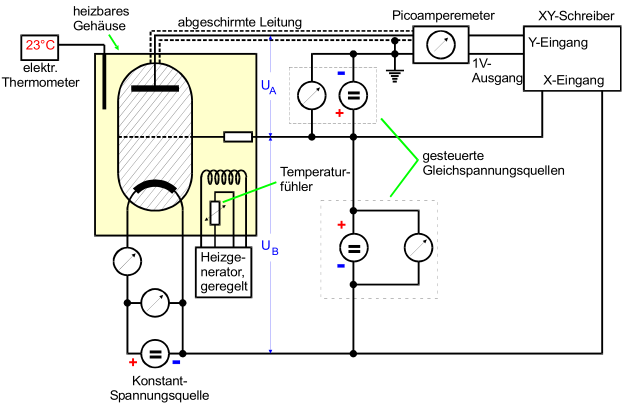
\includegraphics[width=0.75\textwidth]{data/schaltbild.png}
    \caption{Schaltbild des im Versuch verwendeten Aufbaus \cite{Anleitung601}.}
    \label{fig:aufbauSch}
\end{figure}

\noindent
Es wird zu Anfang die integrale Energieverteilung der Elektronen bestimmt. Dazu wird die Beschleunigungsspannung $U_{\text B}$ auf einen konstanten Wert von $\SI{11}{\volt}$ eingetellt und der Auffängerstrom in
Abhängigkeit von der Bremsspannung, die in einem Bereich von $\SIrange{0}{10}{\volt}$ aufgezeichnet wird, gemessen. Die integrale Energieverteilung wird einmal bei Raumtemperatur und zweimal bei erhöhter Temperatur in 
einem Bereich von $\SIrange{140}{160}{\degreeCelsius}$ gemessen. \newline
In einem zweiten Durchführungsschritt werden zwei Franck-Hertz Kurven in einem Temeraturbereich von $\SIrange{160}{200}{\degreeCelsius}$ bei einer konstanten Bremsspannung $U_{\text A}$ von $\SI{1}{\volt}$ in Abhängigkeit 
von der Beschleunigungsspannung von $\SIrange{0}{60}{\volt}$ gemessen. Für die Auswertung wird diejenige Kurve verwendet, die am geeignetsten ist, also die Maxima und Minima am ausgeprägtesten sind.